\documentclass[hide notes]{beamer}
%\documentclass[only notes]{beamer}
\usepackage[english]{babel}
\usepackage{microtype}
\usepackage{environ}
\usepackage{amsmath}
\usepackage[backend=bibtex,style=phys]{biblatex}
\usepackage{doi}
\usepackage{graphicx}
\usepackage{rotating}
\usepackage{tabularx}
\usepackage{dcolumn}
\usepackage{booktabs}
\usepackage{scrextend} % for \footref
\usepackage{hyperref}
\usepackage[nameinlink,capitalize]{cleveref}
\usepackage{siunitx}
\usepackage{floatrow}
\usepackage{bm}
\usepackage{mathtools}

% style stuff
\usetheme{osu}
\hypersetup{hidelinks}
\bibliography{thesis.bib}
% https://tex.stackexchange.com/questions/10102/multiple-references-to-the-same-footnote-with-hyperref-support-is-there-a-bett/10116#10116
\crefformat{footnote}{#2\footnotemark[#1]#3}
% http://tex.stackexchange.com/questions/21913/how-can-i-change-the-footnote-line-thickness-length
\renewcommand{\footnoterule}{%
  \kern -3pt
  \hrule width \textwidth height 0.5pt
  \kern 2pt
}
% http://tex.stackexchange.com/questions/21741/how-do-i-change-footnote-font-size-in-beamer-presentation
\let\oldfootnotesize\footnotesize
\renewcommand*{\footnotesize}{\oldfootnotesize\tiny}
% http://tex.stackexchange.com/questions/169745/left-aligning-footnotes-in-beamer
\makeatletter
\renewcommand<>\beamer@framefootnotetext[1]{%
  \global\setbox\beamer@footins\vbox{%
    \hsize\framewidth
    \textwidth\hsize
    \columnwidth\hsize
    \unvbox\beamer@footins
    \reset@font\footnotesize
    \@parboxrestore
    \protected@edef\@currentlabel
         {\csname p@footnote\endcsname\@thefnmark}%
    \color@begingroup
      \uncover#2{\@makefntext{%
        \rule\z@\footnotesep\ignorespaces\parbox[t]{.9\textwidth}{#1\@finalstrut\strutbox}\vskip1sp}}%
    \color@endgroup}%
}
\makeatother

% custom commands
\DeclareMathOperator{\Tanh}{\mathbf{tanh}}
\DeclarePairedDelimiter\ceil{\lceil}{\rceil}
\DeclarePairedDelimiter\floor{\lfloor}{\rfloor}
% footnote without marker
% https://tex.stackexchange.com/questions/30720/footnote-without-a-marker
\newcommand\blfootnote[1]{%
  \begingroup
  \renewcommand\thefootnote{}\footnote{#1}%
  \addtocounter{footnote}{-1}%
  \endgroup
}

% toc slide
\newcommand\tocframe{%
  \frame{\tableofcontents[currentsection,hideallsubsections]}
}

% use dcolumn
\newcolumntype{d}{D{.}{.}{-1}}
\newcolumntype{e}{D{.}{.}{8}}
\newcolumntype{f}{D{.}{.}{13}}

\title{Essential Reservoir Computing}
%\subtitle{}

\author[Griffith]{Aaron Griffith}
\institute[Ohio State University]{Department of Physics\\Ohio State University}
\date[8/17/2021]{August 17, 2021}

\begin{document}

\begin{frame}[plain]
  \titlepage
\end{frame}

%\setbeamertemplate{footline}[frame number]{\tiny\insertframenumber\,/\,\inserttotalframenumber}
% https://tex.stackexchange.com/questions/434923/frame-number-does-not-work-since-ubuntu-update?noredirect=1&lq=1
\setbeamertemplate{navigation symbols}{\textcolor{osured}{\tiny\insertframenumber\,/\,\inserttotalframenumber}}

\section{Introduction}
% why RC? use word 'examples'

\frame{\tableofcontents[hideallsubsections]}

\begin{frame}{Machine Learning and Neural Networks}
  \begin{columns}
    \column{0.5\textwidth}
    \begin{itemize}
    \item neural networks are universal models
    \item learn relationship between input and output from example data
    \item very useful if this relationship is unknown, but examples are easy to find
    \item canonical example: learn how to turn images of digits into labels
    \end{itemize}
    \column{0.5\textwidth}
    \centering
    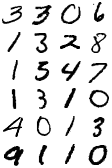
\includegraphics[width=0.7\textwidth]{figures/mnist.png}
  \end{columns}
\end{frame}

\begin{frame}{Machine Learning in Physics}
  \begin{itemize}
  \item Elsewhere:
    \begin{itemize}
    \item find masses of particles from decay data\footnote{\fullcite{lonnblad1992}}
    \item separate quark and gluon jets in $e^+ e^-$ annihilation\footnote{\fullcite{csabai1991}}
    \end{itemize}
  \item In this presentation:
    \begin{itemize}
    \item \textbf{system state inference}: given $x(t)$ and $y(t)$, find $z(t)$
    \item \textbf{chaotic system forecasting}: given the beginning of a signal $u(t)$, what happens after?
    \end{itemize}
  \end{itemize}
\end{frame}

\begin{frame}{Chaotic System Forecasting}
  \centering
  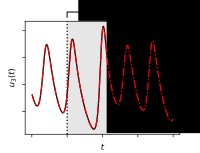
\includegraphics[width=0.7\textwidth]{figures/prediction-example}
\end{frame}

\begin{frame}{The Problem with Neural Networks}
  \begin{itemize}
  \item very expensive to train
    \begin{itemize}
    \item data hungry: require many examples
    \item deep networks take longer to train: ``vanishing gradient problem''
    \end{itemize}
  \item alternative: \textbf{Reservoir Computers}
    \begin{itemize}
    \item quick training
    \item physical interpretation
    \item physical implementation
    \end{itemize}
  \end{itemize}
\end{frame}

\section{Reservoir Computing}

\tocframe

\begin{frame}{Reservoir Computers}
  \begin{itemize}
  \item RC transforms an input signal $\bm{u}(t)$ into an output $\bm{y}(t)$
  \item input $\bm{u}(t)$ acts as driving input to dynamical system $\bm{R}$ \\ (the ``reservoir''),
    $$ \dot{\bm{r}}(t) = \bm{R}(\bm{r}, \bm{u}, t) $$
  \item reservoir response $\bm{r}(t)$ is read-out via $\bm{g}$, and linearly combined into output
    $$ \bm{y}(t) = W_\text{out}\;\bm{g}\left(\bm{r}\left(t\right)\right) $$
  \item reservoir $\bm{R}$ and read-out $\bm{g}$ fixed ahead of time, but $W_\text{out}$ is trained to fit example data
  \end{itemize}
\end{frame}

\begin{frame}{Reservoir Computers}
  \centering
  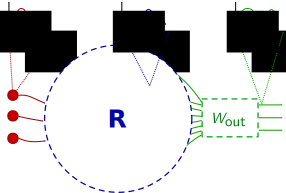
\includegraphics[width=0.8\textwidth]{figures/reservoir-generic}
\end{frame}

\begin{frame}{Training an RC}
  \begin{itemize}
  \item use example input $\bm{u}_\text{train}(t)$ and example output $\bm{y}_\text{train}(t)$
  \item example input produces example reservoir response $\bm{r}_\text{train}(t)$
  \item Goal: find $W_\text{out}$ such that
    $$ \bm{y}_\text{train}(t) \approx W_\text{out}\;\bm{g}\left(\bm{r}_\text{train}\left(t\right)\right)$$
  \item this is \emph{linear regression}! this is \emph{fast}!
  \item usually, RCs use ridge regression
  \end{itemize}
\end{frame}

\begin{frame}{Forecasting with an RC}
  \begin{itemize}
  \item for system forecasting, find $W_\text{out}$ such that
    $$ \bm{u}_\text{train}(t) \approx W_\text{out}\;\bm{g}\left(\bm{r}_\text{train}\left(t\right)\right)$$
  \item after training, feed output of RC back into itself as input
  \end{itemize}
  \centering
  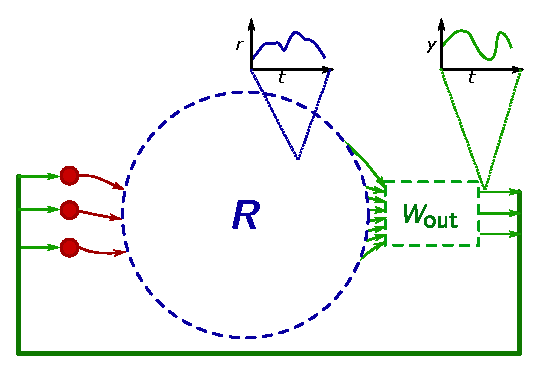
\includegraphics[width=0.6\textwidth]{figures/reservoir-predict}
\end{frame}

\begin{frame}{Evaluating an RC}
  \begin{itemize}
  \item use normalized root-mean-squared error (NRMSE),
    $$ \epsilon = {\left(\sum_i\frac{\int \left| y_i(t) - y_{\text{test},i}(t) \right|^2 \;dt}{T \operatorname{Var}\left[y_{\text{test},i}(t)\right]}\right)}^{1/2} $$
  \item for chaotic system forecasting, a forecast \emph{must} diverge eventually, so only calculate for 1 Lyapunov period ($\epsilon_1$)
  \item if forecasting starts near an unstable part of the input system, small errors will amplify and $\epsilon_1$ is misleading
  \item instead, perform $m$ forecasts and average the errors
    $$ \tilde{\epsilon} = {\left( \frac{1}{m} \sum_{i=1}^m \epsilon_{1,i}^2 \right)}^{1/2} $$
  \end{itemize}
\end{frame}

\begin{frame}{Evaluating an RC}
  \centering
  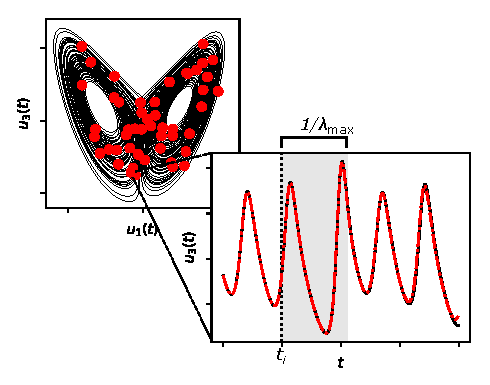
\includegraphics[width=0.8\textwidth]{figures/nrmse-avg}
\end{frame}

\begin{frame}{Echo State Networks}
  \begin{itemize}
  \item use an \emph{untrained} neural network as reservoir
  \item $N$ exponential decay nodes
  \item each node has inputs drawn from $u(t)$ or other nodes
  \item summed inputs pass through activation function $f$ to drive exponential
  \end{itemize}
  \centering
  \begin{align*}
    \dot{\bm{r}}(t) &= - \gamma \bm{r}(t) + \gamma \bm{f}\left( W_r\;\bm{r}(t) + W_\text{in}\;\bm{u}(t) \right) \\
    \bm{y}(t) &= W_\text{out}\;\bm{g}\left(\bm{r}(t)\right)
  \end{align*}
\end{frame}

\begin{frame}{Echo State Networks}
  \centering
  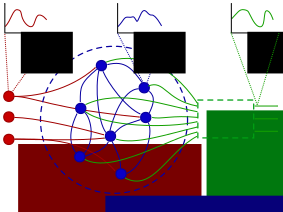
\includegraphics[width=0.8\textwidth]{figures/reservoir}
\end{frame}

\begin{frame}{Constructing ESNs}
  \begin{itemize}
  \item $\gamma$ (node decay rate) is tuned to match input timescale
  \item $f$ (activation function) is traditionally $\tanh$
    \vspace{2em}
  \item $W_r$ and $W_\text{in}$ chosen \emph{randomly}
    \begin{itemize}
    \item $k$, recurrent inputs for each node
    \item $\rho_r$, spectral radius of $W_r$
    \item $\sigma$, probability of external input per node
    \item $\rho_\text{in}$, scale of $W_\text{in}$
    \end{itemize}
    \vspace{2em}
  \item What reservoirs work well? What ESN parameters work well?
  \item \emph{How much of this is necessary?}
  \end{itemize}
\end{frame}

\section{Low-Connectivity Reservoirs}

\tocframe

\begin{frame}{Exploring ESN Parameters}
  \begin{columns}
    \column{0.6\textwidth}
    \begin{itemize}
    \item use Bayesian optimization to find ESN parameters that work well for Lorenz system forecasting
    \item strange result: optimized parameters often had $k = 1$
    \item ESNs with $k = 1$ have very simple structure, but perform as well as $k > 1$
    \item inspired by this, I also look at three other simple structures...
    \end{itemize}
    \column{0.4\textwidth}
    \centering
    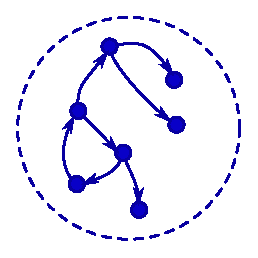
\includegraphics[width=1.0\textwidth]{figures/topology-b}
  \end{columns}
\end{frame}

\begin{frame}{Structure of Low-Connectivity Reservoirs}
    \begin{columns}
      \column{0.4\textwidth}
      \small
      (a) general construction \\
      (b) $k = 1$, single cycle \\
      (c) $k = 1$, cut cycle \\
      (d) \emph{simple cycle reservoir}\footnote[frame]{\fullcite{rodan2011}\label{fn:rodan}} \\
      (e) \emph{delay line reservoir}\cref{fn:rodan} \\~\\
      In all cases, networks with more than one connected component are discarded and regenerated
      \column{0.6\textwidth}
      \centering
      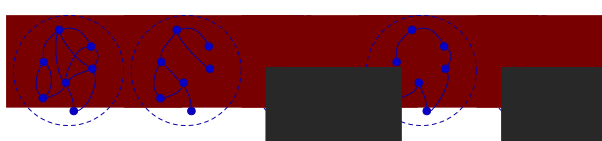
\includegraphics[width=1.0\textwidth]{figures/topology}
  \end{columns}
\end{frame}

\begin{frame}{Training, Forecasting, and Evaluation}
  \begin{itemize}
  \item for each structure, I search for the parameters to optimize $\tilde{\epsilon}$ on Lorenz forecasting
  \item for each set of trial parameters...
    \begin{itemize}
    \item build a 100-node ESN with those parameters
    \item train for 100 units of time ($\Delta t = 0.01$)
    \item evaluate $\tilde{\epsilon}$ by averaging $50$ $\epsilon_1$ errors
    \end{itemize}
    \vspace{2em}
  \item in the end, have one ESN from each structure type that performs well
  \end{itemize}
\end{frame}

\begin{frame}{ESN Symmetries and their Consequences}
  \begin{itemize}
  \item when $f = \tanh$ and $\bm{g}(\bm{r}) = \bm{r}$, ESN equation has $\bm{r} \rightarrow -\bm{r}$ symmetry, and therefore $\bm{y} \rightarrow -\bm{y}$ symmetry
    \begin{align*}
      \dot{\bm{r}}(t) &= - \gamma \bm{r}(t) + \gamma \bm{f}\left( W_r\;\bm{r}(t) + W_\text{in}\;\bm{u}(t) \right) \\
      \bm{y}(t) &= W_\text{out}\;\bm{g}\left(\bm{r}(t)\right)
    \end{align*}
  \item Lorenz does \emph{not}!
  \item Solution: break the symmetry by using a non-linear $\bm{g}$\footnote{\fullcite{herteux2020}}
    \begin{equation*}
      g_i(\bm{r}) = \begin{cases}
        r_i & \text{if } i \leq N / 2, \\
        r_i^2 & \text{if } i > N / 2.
      \end{cases}
    \end{equation*}
    \end{itemize}
\end{frame}

\begin{frame}{ESN Symmetries and their Consequences}
  \centering
  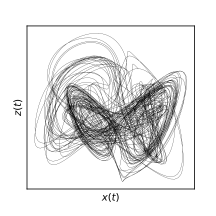
\includegraphics[width=0.7\textwidth]{figures/lorenz-symmetry}
\end{frame}

\begin{frame}{$\epsilon_1$ vs. $\tilde{\epsilon}$}
  \begin{center}
    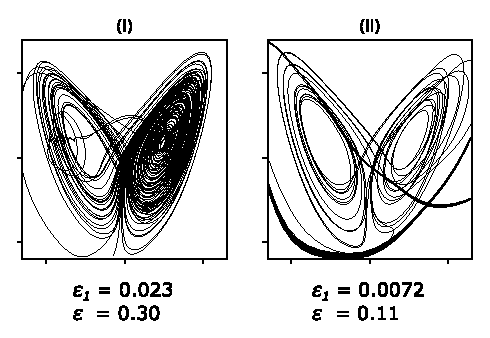
\includegraphics[width=0.7\textwidth]{figures/epsilon-failure}
  \end{center}

  {\small
    (i) overemphasizes lobe where $\epsilon_1$ resides \\
    (ii) good short-term forecast, but falls into periodic orbit as $t \rightarrow \infty$}
\end{frame}

\begin{frame}{Results}
  \centering
  \begin{tabularx}{\linewidth}{l l@{\extracolsep{\fill}} l}
    & Structure & $\tilde{\epsilon}$ \\
    \hline
    (a) & Any $k$ & 0.022 $\pm$ 0.004 \\
    (b) & $k = 1$ with cycle & 0.024 $\pm$ 0.005 \\
    (c) & $k = 1$ no cycle & 0.028 $\pm$ 0.005$^*$ \\
    (d) & cycle & 0.023 $\pm$ 0.008 \\
    (e) & line & 0.024 $\pm$ 0.003$^*$ \\
  \end{tabularx}

  \vspace{3em}
  $^*$ \emph{no recurrence in network!}
\end{frame}

\begin{frame}{Results}
  \centering
  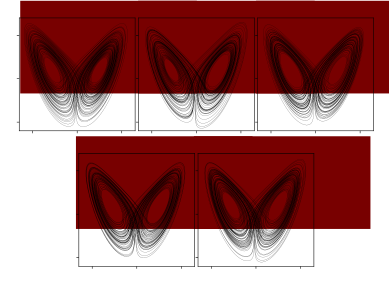
\includegraphics[width=0.7\textwidth]{figures/lowk-attractors}
\end{frame}

\begin{frame}{ESN Variation}
  \begin{itemize}
    \item ESN construction is random -- what if I re-generate a network with the same parameters as best performers?
  \end{itemize}
  \centering
  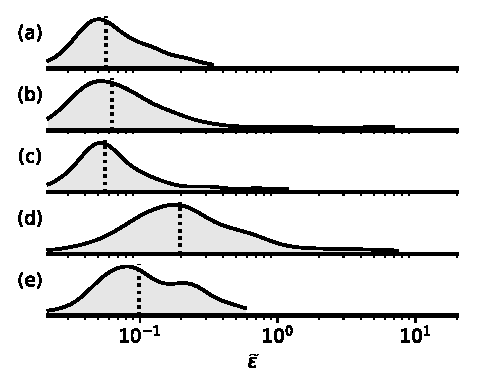
\includegraphics[width=0.7\textwidth]{figures/epsilon-distribution}
\end{frame}

\begin{frame}{Conclusion}
  \begin{itemize}
  \item $\tilde{\epsilon}$ captures forecasting quality more reliably than $\epsilon_1$
  \item very simple ESNs can perform as well as ESNs with more complicated connectivity
  \item this is still true even when the network is a single cycle, or a line
  \item however, well-performing simple ESNs are harder to find
    \vspace{3em}
  \item If line networks work well... maybe all the network does is combine time-delayed copies of the input?
  \end{itemize}
\end{frame}

\section{RCs without Reservoirs: NVARs}

\tocframe

\begin{frame}{NVARs are equivalent to ESNs}
  \begin{itemize}
  \item in 2020, Erik Bollt proved that a linear ESN ($f$ and $\bm{g}$ both identity functions) is equivalent to a \emph{vector auto-regression} (VAR)
  \item shortly after, he extended this proof to equivalence between output-nonlinear ESNs ($\bm{g}$ nonlinear) and nonlinear VARs
    \vspace{2em}
  \item a full mathematical equivalence proof that (at least some) ESNs are exactly equivalent to combining time-delayed copies of the input!\usebeamercolor[fg]{frametitle}{!!}
    \blfootnote{\fullcite{bollt2021}}
  \end{itemize}
\end{frame}

\begin{frame}{Nonlinear VARs}
  \begin{itemize}
  \item transforms an input $\bm{u}(t)$ into output $\bm{y}(t)$
  \item given a time step $\Delta t$ and tap delays $\tau_0, \dots, \tau_{q-1}$, build
    $$ \bm{v}(t + \Delta t) = \bm{u}(t - \tau_0 \Delta t) \oplus \bm{u}(t - \tau_1 \Delta t) \oplus \cdots \oplus \bm{u}(t - \tau_{q-1} \Delta t) $$
  \item construct the output from a nonlinear function of $\bm{v}$,
    $$ \bm{y}(t + \Delta t) = W_\text{out}\;\bm{g}_\text{n}\left(\bm{v}(t + \Delta t)\right) $$
    \vspace{2em}
    \item note similarity to RC approach: replace $\bm{r}(t)$ with $\bm{v}(t)$, and $\bm{g}(\bm{r})$ with $\bm{g}_\text{n}(\bm{v})$
  \end{itemize}
\end{frame}

\begin{frame}{Nonlinear VARs}
  \centering
  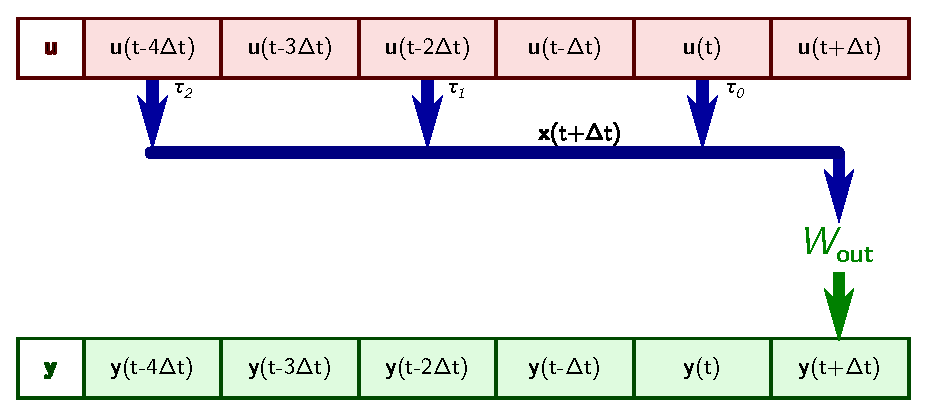
\includegraphics[width=0.9\textwidth]{figures/var-infer}
\end{frame}

\begin{frame}{Training and Testing}
  \begin{itemize}
  \item same process as for RCs!
  \item feed in example input $\bm{u}_\text{train}(t)$ to produce $\bm{v}_\text{train}(t)$, then use ridge regression to find $W_\text{out}$
  \item for forecasting, connect output to input as with RCs, but modify output slightly
    $$ \bm{y}(t + \Delta t) = \bm{u}(t) + W_\text{out}\;\bm{g}_\text{n}\left(\bm{v}(t + \Delta t)\right) $$
  \item testing also uses NRMSE $\epsilon$ and $\tilde{\epsilon}$
  \end{itemize}
\end{frame}

\begin{frame}{$\bm{g}$ vs. $\bm{g}_\text{n}$}
  \begin{itemize}
  \item important: under equivalence, the $\bm{g}$ of the ESN is \emph{not} identical to $\bm{g}_\text{n}$
  \item for an ESN with quadratic readout $\bm{g}(\bm{r})$
    \begin{equation*}
      g_i(\bm{r}) = \begin{cases}
        r_i & \text{if } i \leq N, \\
        r_{i - N}^2 & \text{if } N < i \leq 2N.
      \end{cases}
    \end{equation*}
  \item equivalent NVAR $\bm{g}_\text{n}(\bm{v})$ has all possible linear and quadratic terms of components of $\bm{v}$
    $$ \bm{g}_\text{n}(\bm{v}) = \bm{v} \oplus \ceil{\bm{v} \otimes \bm{v}} $$
  \item this suggests an easy extension: keep adding higher order terms to $\bm{g}_\text{n}$ until NVAR works
  \end{itemize}
\end{frame}

\begin{frame}{Practical Considerations}
  \begin{itemize}
  \item NVARs are equivalent to ESNs, but completely sidestep the issue of choosing a network
  \item replace reservoir with simple time-delay taps
  \item why ever use an ESN if an NVAR will work?
    \vspace{2em}
  \item for $q$ taps, $d$ input dimensions, and $n$-degree polynomial terms, $W_\text{out}$ has to fit $(qd)^n$ components
  \item mathematically, equivalence only holds for \emph{infinite taps} ($q \rightarrow \infty$)
  \item are NVARs still useful for low $q$ and low $n$?
  \end{itemize}
\end{frame}

\section{NVARs in Practice}

\tocframe

\begin{frame}{NVARs in Practice}
  Low-tap, low-degree NVARs perform well on
  \begin{itemize}
  \item Lorenz '63 state inference
  \item Lorenz '63 forecasting
  \item double-scroll circuit forecasting
  \item Mackey-Glass forecasting
  \end{itemize}
\end{frame}

\begin{frame}{Lorenz '63 State Inference}
  \begin{itemize}
  \item Goal: infer Lorenz $z$ from $x$ and $y$
  \item four taps, $\tau_0 = 0$, $\tau_1 = 5$, $\tau_2 = 10$, $\tau_3 = 15$
  \item $\Delta t = 0.05$ (20 points per Lyapunov period)
  \item $\bm{g}_\text{n}$ includes constant, linear, and quadratic terms
    $$ \bm{g}_\text{n}(\bm{v}) = 1 \oplus \bm{v} \oplus \ceil{\bm{v} \otimes \bm{v}} $$
  \item train on 20 time units (400 data points)
  \item evaluate on 45 time units (900 data points)
  \end{itemize}
\end{frame}

\begin{frame}{Lorenz '63 State Inference Results}
  \begin{center}
    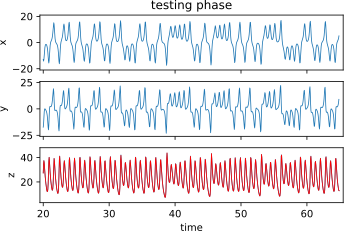
\includegraphics[width=0.8\textwidth]{figures/nvar-infer-lorenz-testing}
  \end{center}
  \begin{itemize}
  \item NRMSE $\epsilon = 1.75\pm0.3\times10^{-2}$
  \end{itemize}
\end{frame}

\begin{frame}{Lorenz '63 Forecasting}
  \begin{itemize}
  \item Goal: forecasting on Lorenz $x$, $y$, and $z$
  \item two taps, $\tau_0 = 0$ and $\tau_1 = 1$
  \item $\Delta t = 0.025$ (40 points per Lyapunov period)
  \item $\bm{g}_\text{n}$ includes constant, linear, and quadratic terms
    $$ \bm{g}_\text{n}(\bm{v}) = 1 \oplus \bm{v} \oplus \ceil{\bm{v} \otimes \bm{v}} $$
  \item train on 10 time units (400 data points)
  \item evaluate $\tilde{\epsilon}$ with 10 trials of $\epsilon_1$
  \end{itemize}
\end{frame}

\begin{frame}{Lorenz '63 Forecasting Results}
  \begin{center}
    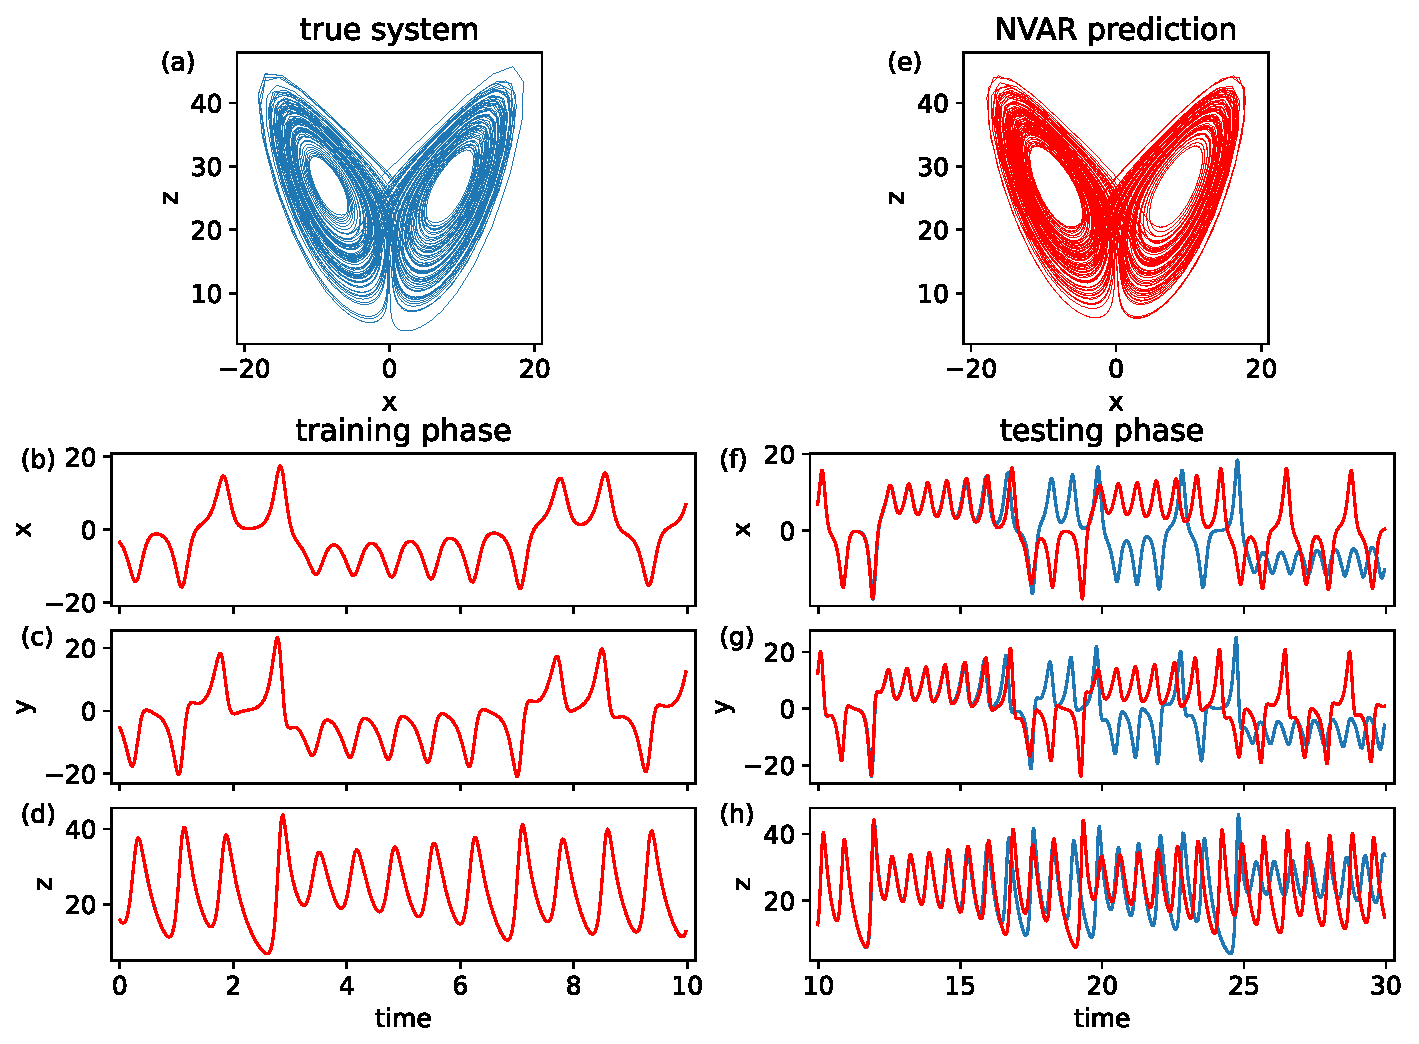
\includegraphics[width=0.8\textwidth]{figures/nvar-predict-lorenz}
  \end{center}
  \begin{itemize}
  \item NRMSE $\tilde{\epsilon} = 4.51\pm0.85\times10^{-3}$
  (~5$\times$ better than ESNs earlier!)
  \end{itemize}
\end{frame}

% put rmap here if needed

\begin{frame}{Lorenz '63 Forecasting $W_\text{out}$}
  \begin{columns}
    \column{0.4\textwidth}
    \begin{itemize}
    \item Lorenz vector field is quadratic
    \item is NVAR only working because it has matching quadratic terms?
    \item \textbf{No.} Terms in Lorenz (in red) are not favored over others.
    \end{itemize}
    \column{0.6\textwidth}
    \centering
    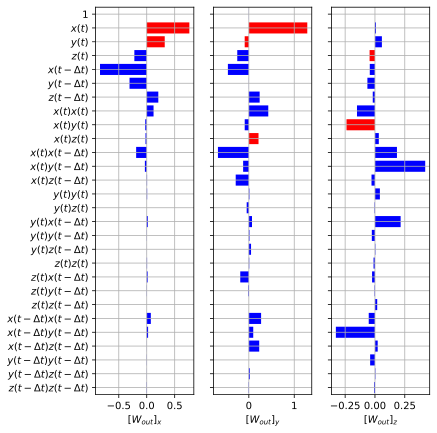
\includegraphics[width=1.0\textwidth]{figures/nvar-predict-lorenz-wout}
  \end{columns}
\end{frame}

\begin{frame}{Double-Scroll Forecasting}
  \begin{itemize}
  \item Goal: forecasting for double-scroll circuit
  \item two taps, $\tau_0 = 0$ and $\tau_1 = 1$
  \item $\Delta t = 0.25$ (40 points per Lyapunov period)
  \item $\bm{g}_\text{n}$ includes linear and cubic terms, to match symmetry
    $$ \bm{g}_\text{n}(\bm{v}) = \bm{v} \oplus \ceil{\bm{v} \otimes \bm{v} \otimes \bm{v}} $$
  \item train on 100 time units (400 data points)
  \item evaluate $\tilde{\epsilon}$ with 10 trials of $\epsilon_1$
  \end{itemize}
\end{frame}

\begin{frame}{Double-Scroll Forecasting Results}
  \begin{center}
    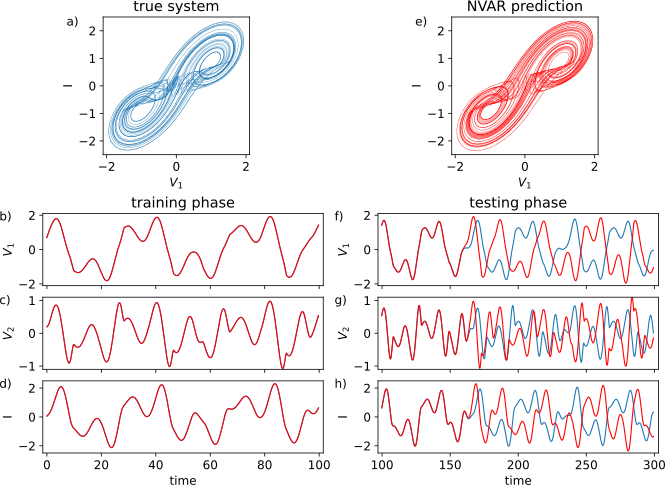
\includegraphics[width=0.8\textwidth]{figures/nvar-predict-dscroll}
  \end{center}
  \begin{itemize}
  \item NRMSE $\tilde{\epsilon} = 2.15\pm0.63\times10^{-2}$
  (~1.5$\times$ better)
  \end{itemize}
\end{frame}

\begin{frame}{Mackey-Glass Forecasting}
  \begin{itemize}
  \item Goal: forecasting for Mackey-Glass system
  \item four taps, $\tau_0 = 0$, $\tau_1 = 1$, $\tau_2 = \floor{17/2\Delta t}$, $\tau_3 = \tau_2 + 1$
  \item $\Delta t = 0.2$ (500 points per Lyapunov period)
  \item $\bm{g}_\text{n}$ includes constant up to cubic terms
    $$ \bm{g}_\text{n}(\bm{v}) = 1 \oplus \bm{v} \oplus \ceil{\bm{v} \otimes \bm{v}} \oplus \ceil{\bm{v} \otimes \bm{v} \otimes \bm{v}} $$
  \item train on 1000 time units (5000 data points\emph{!})
  \item evaluate $\tilde{\epsilon}$ with 10 trials of $\epsilon_1$
  \end{itemize}
\end{frame}

\begin{frame}{Mackey-Glass Forecasting Results}
  \begin{center}
    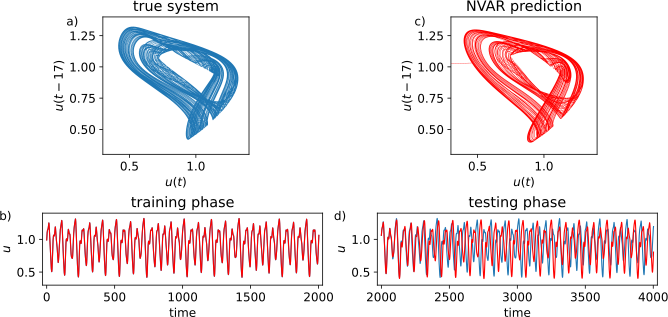
\includegraphics[width=0.8\textwidth]{figures/nvar-predict-mackey-glass}
  \end{center}
  \begin{itemize}
  \item NRMSE $\tilde{\epsilon} = 5.77\pm0.42\times10^{-2}$
  \end{itemize}
\end{frame}

\begin{frame}{Conclusion}
  \begin{itemize}
  \item NVARs have comparable performance to ESNs on Lorenz '63 and double-scroll circuit
  \item only need a few taps and low-order nonlinearity
  \item careful tap positioning can aid in keeping number of taps low
    \vspace{2em}
  \item not quite as great on Mackey-Glass
  \item $\bm{g}_\text{n}$ needs access to higher order terms without exponential explosion in size of $W_\text{out}$
  \item possible future research: using full nonlinear functions, rather than monomial terms
  \end{itemize}
\end{frame}

\section{Conclusion}

\tocframe

\begin{frame}
  \begin{center}
    {\usebeamercolor[fg]{frametitle}{\Large Thank you!}}

    Questions?
  \end{center}

  \note{o7}
\end{frame}

\end{document}

